Consider the air-pollution data given in Table 1.5. Construct a \textit{Q-Q} plot for the solar
radiation measurements and carry out a test for normality based on the correlation
coefficient $r_{Q}$ [see (4--31)]. Let $\alpha = .05$ and use the entry corresponding to $n = 40$ in Table 4.2.

\begin{figure}[H]
    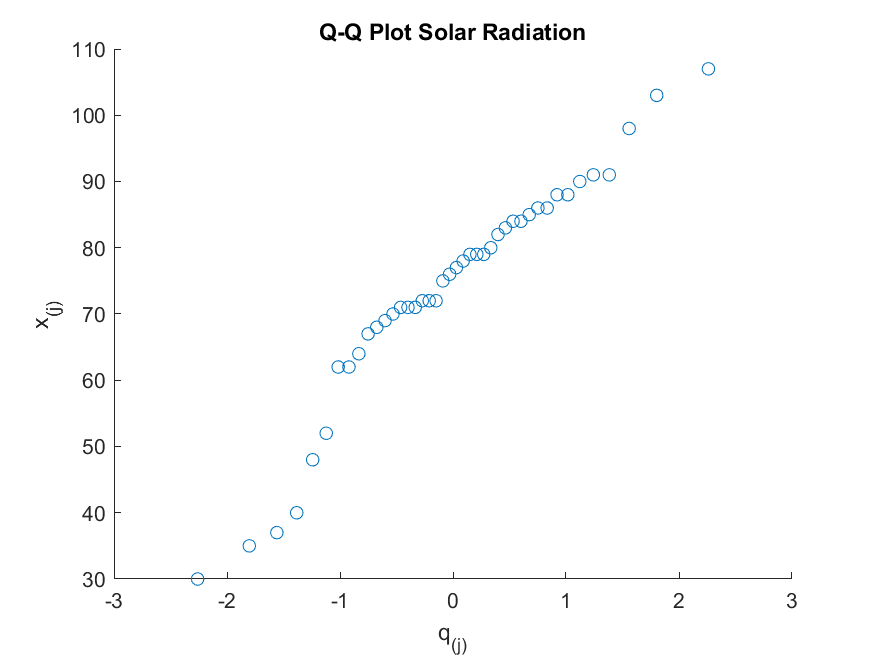
\includegraphics[scale=0.8]{./matlab/chapter-4/sol4.28.png}
\end{figure}

The correlation coefficient for the data is $r_{Q} = \text{Corr}(q_{(j)}, x_{(j)}) = 0.9693$. The value in Table 4.2 when n=40 and $\alpha = 0.05$ is 0.9726. Our value of $R_{Q}$ is less than the value in the table, so we'd conclude that the data is normally distributed.